\section{Evaluation}
\label{chap:evaluation}
In der letzten Phase unseres Projekts wurde uns ein Framework des SAFEST-Projekts zur Verfügung gestellt, welches die Möglichkeit bietet, verschiedene Algorithmen miteinander zu vergleichen. Das Framework erhält als Eingabe eine Matrix, in der Vordergrundobjekte durch den zu testenden  Algorithmus markiert sind, und berechnet im Folgenden basierend auf vordefinierten Abstandsparametern, die die Größe eines Menschen beschreiben, die Anzahl von Personen im Bild zu einem bestimmten Zeitpunkt.

Nach der Integration unseres Algorithmus in das Framework wird eine vergleichende Analyse mit der vorimplementierten, Histogramm-basierten Lösung durchgeführt. Als Metrik verwenden wir hierbei den Abstand zur tatsächlichen Anzahl von Personen im Bild. Die erwarteten Werte für diesen Vergleich sind uns seitens des SAFEST Projekts zur Verfügung gestellt worden und wurden manuell ermittelt. Das Ergebnis haben wir visualisiert, indem wir jeweils die Abweichung vom eigentlich erwarteten Wert als Graph dargestellt haben. Ein optimal funktionierender Algorithmus würde demnach als Graph im Diagramm ohne Abweichungen die Nulllinie verdecken. Es werden drei Videos von unterschiedlichen Umgebungen untersucht.\\
Im Folgenden werden die zwei Algorithmen wie folgt benannt:
\begin{description}
	\item[Histogramm)] die bereits implementierte Lösung, die mit Histogrammen arbeitet
	\item[HMM)] unsere HMM-basierte Lösung, wobei zunächst mit einem Video gelernt wird und dann die Analyse auf einem zweitem Video der selben Szenerie statt findet
\end{description}
Weitere Vergleiche haben wir nicht angestellt, da das Histogramm-basierte Verfahren den anderen Verfahren entweder überlegen ist (OpenCV MOG und OpenCV MOG2) oder aber das Verfahren den Hintergrund hart auf bestimmte Videos kodiert (MEAN) und sehr unflexibel ist, sobald der Hintergrund nicht mehr uniform ist.

\subsection{Vergleich mit Histogramm-basierter Implementierung: Innenhof}
\label{sec:eval_innenhof}

\begin{figure}
	\centering
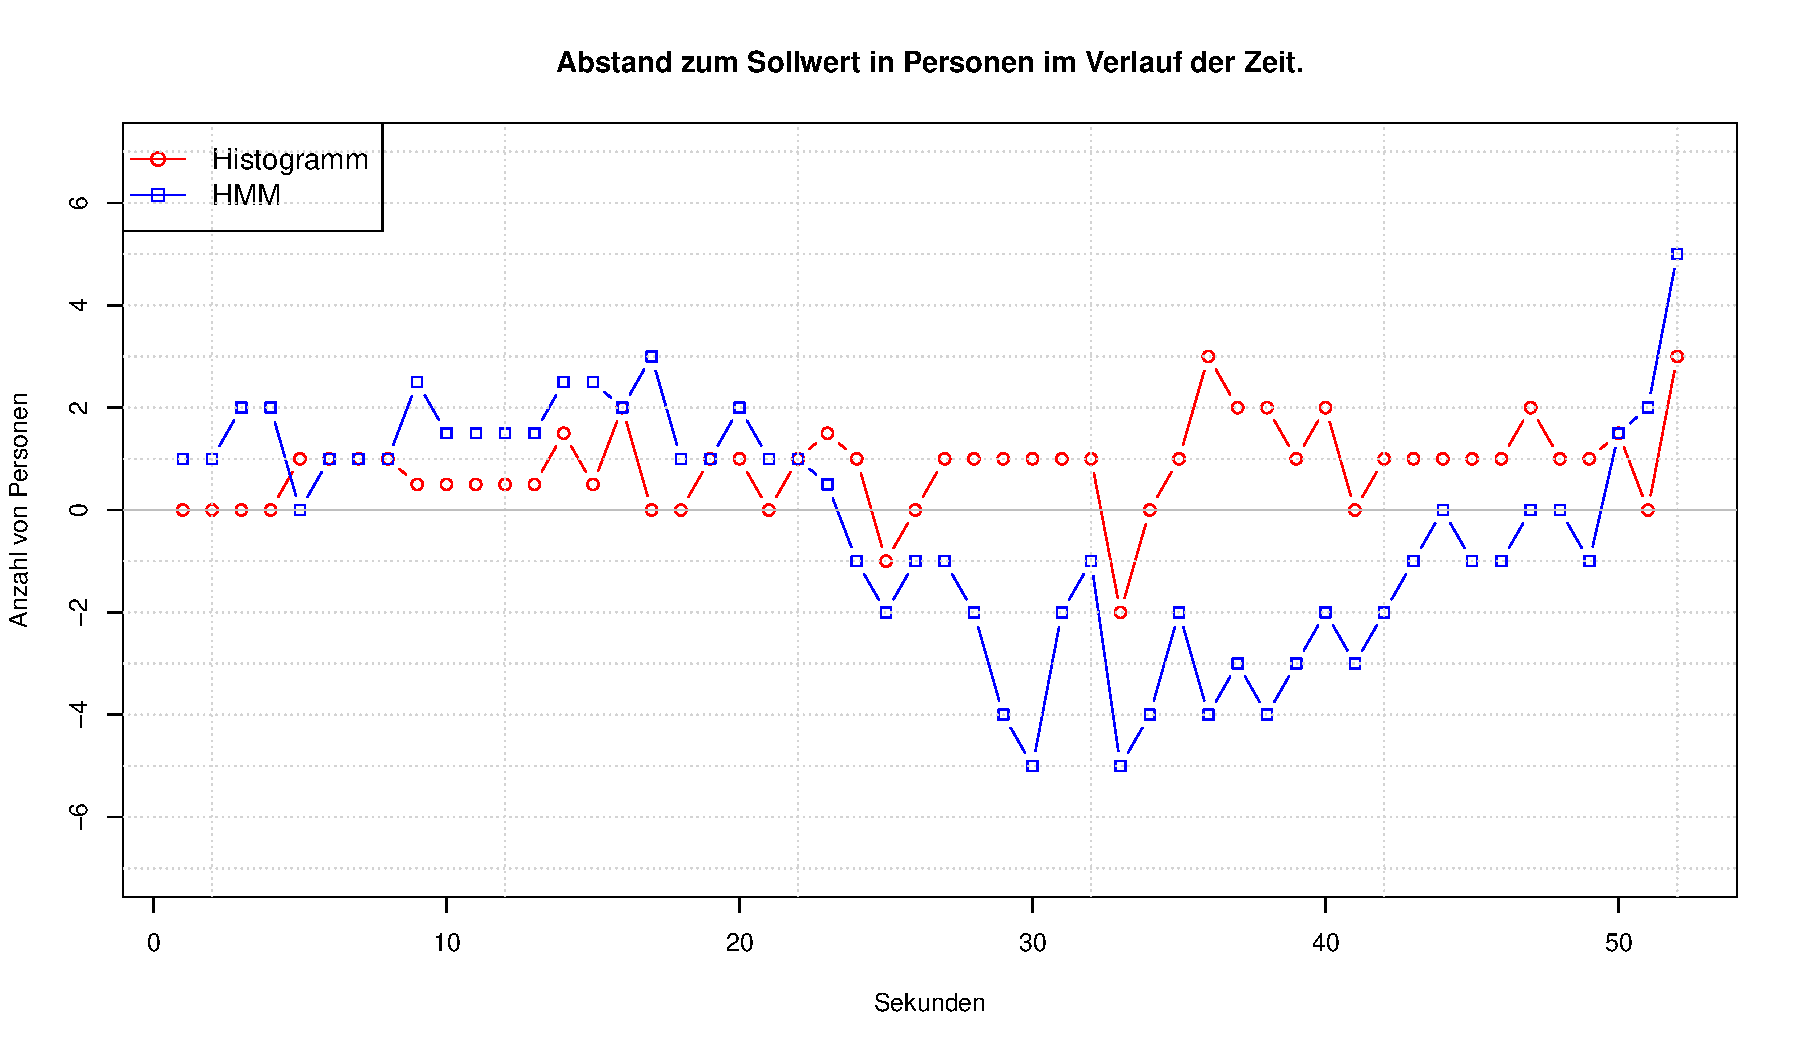
\includegraphics[width=1\textwidth]{bilder/innenhof_910-1000_histo_vs_hmm_prelearned.pdf}
\caption{Innenhof: Histogramm vs. trainiertes HMM}
	\label{fig:Innenhof}
\end{figure}

Abbildung \ref{fig:Innenhof} zeigt auf, dass der Histogramm-basierte Algorithmus für dieses Video durchgehend bessere Ergebnisse liefert, als der HMM-basierte Algorithmus. Der HMM-Algorithmus ist im Durchschnitt 1-2 Personen weiter vom realen Wert entfernt als sein Konkurrent. Im Besonderen gilt dies für den zweiten Teil des Videos.

\subsection{Vergleich mit Histogramm-basierter Implementierung: Tegel}
\label{sec:eval:tegel}

\begin{figure}
	\centering
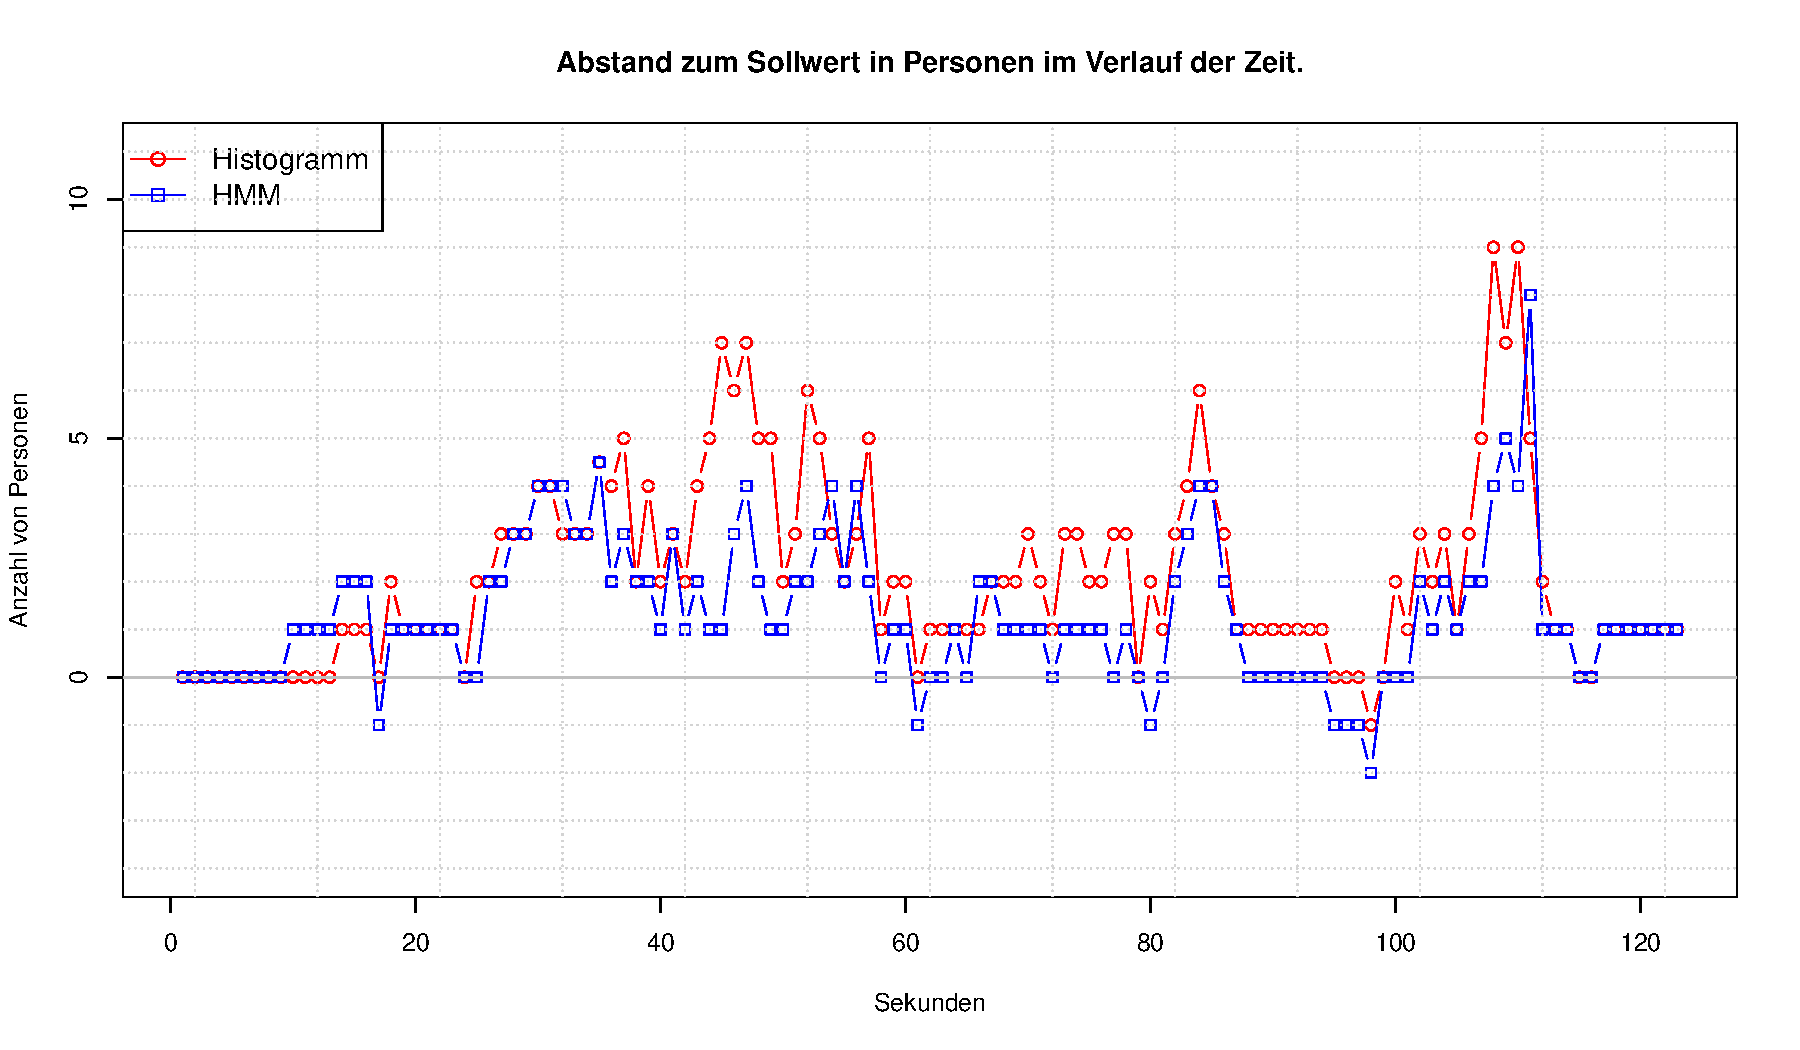
\includegraphics[width=1\textwidth]{bilder/tegel_7-55_histo_vs_prelearned_hmm.pdf}
	\caption{Tegel: Histogramm vs. trainiertes HMM}
	\label{fig:tegel}
\end{figure}

Wie man der Abbildung \ref{fig:tegel} entnehmen kann, sind die Ergebnisse beider Algorithmen vom Verlauf her sehr ähnlich, allerdings weist der HMM-basierte Algorithmus gegenüber dem Histogramm-basierten kleine Vorteile auf.
Zwischen 30 und 50 Sekunden hat er eine deutlich geringere Abweichung vom korrekten Wert. Dasselbe gilt für den Bereich zwischen ca. 65 und 80 Sekunden.\\

\subsection{Vergleich mit Histogramm-basierter Implementierung: Eingang}
\label{sec:eval_eingang}

\begin{figure}
	\centering
	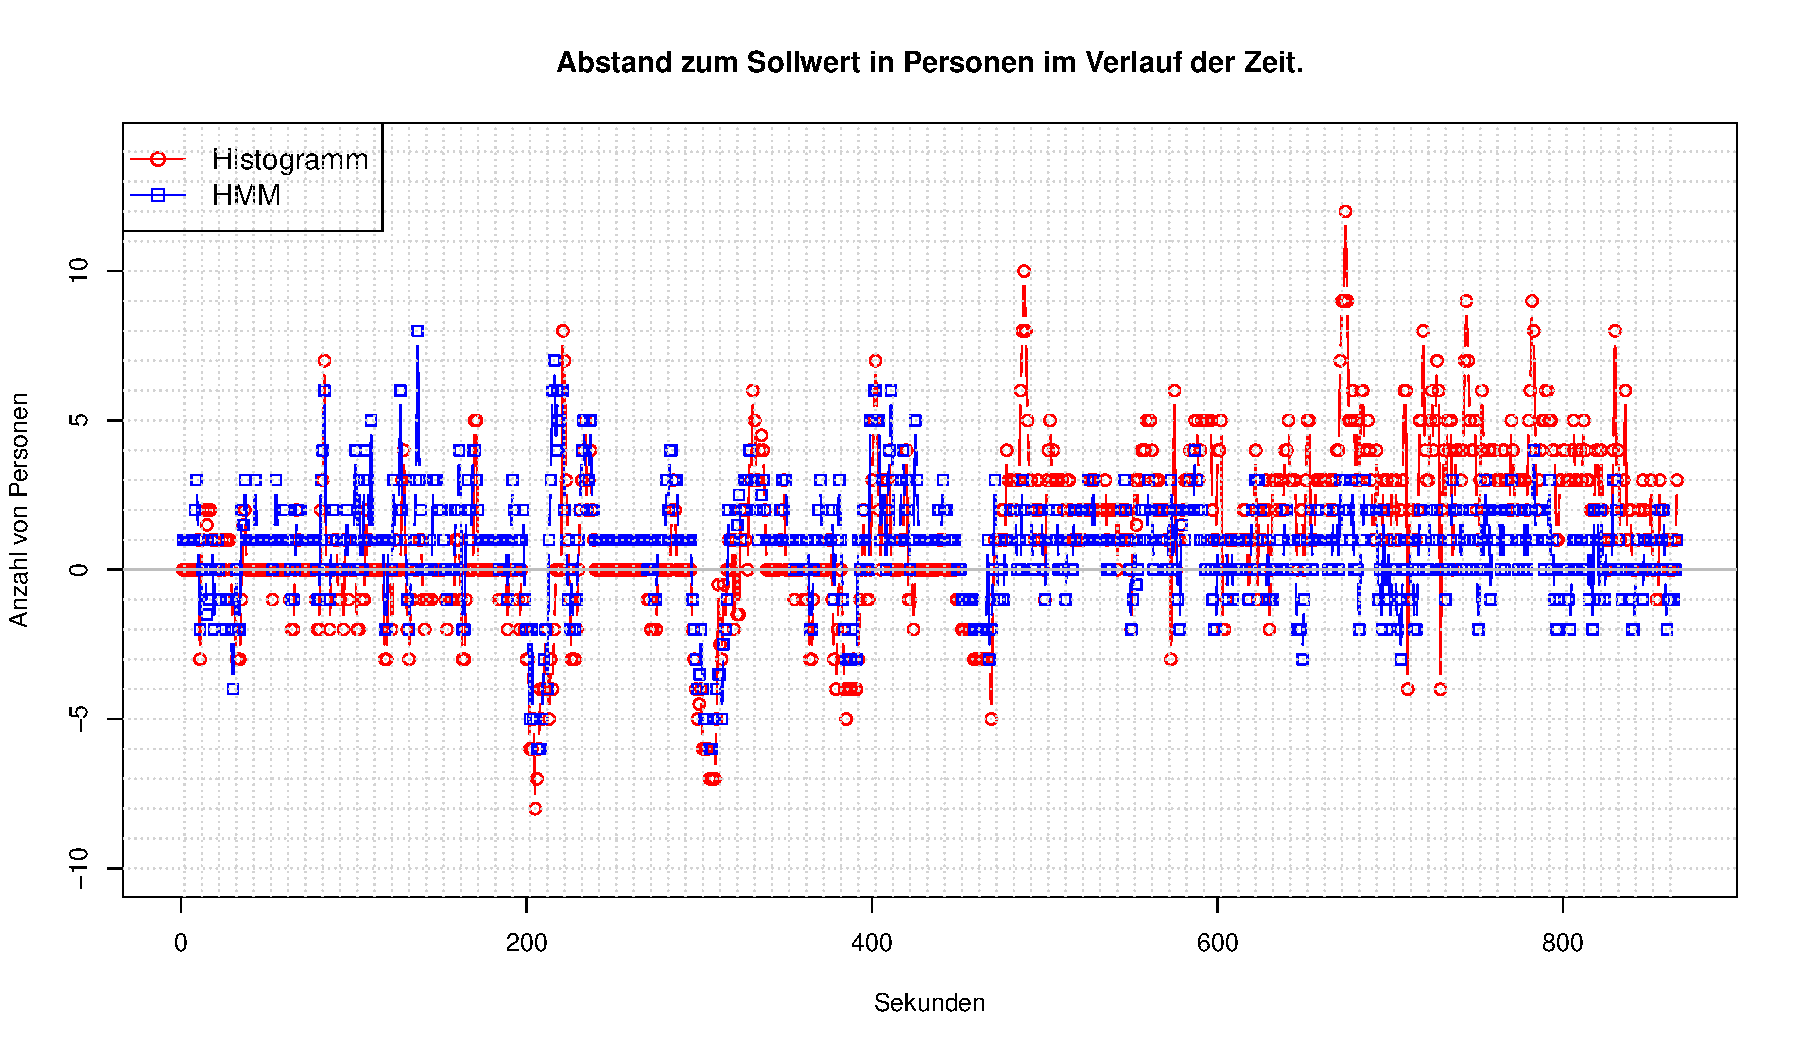
\includegraphics[width=1\textwidth]{bilder/eingang2_histo_vs_hmm_prelearned.pdf}
	\caption{Eingang: Histogramm vs. trainiertes HMM (gesamt)}
	\label{fig:Eingang-gesamt}
\end{figure}

\begin{figure}
	\centering
	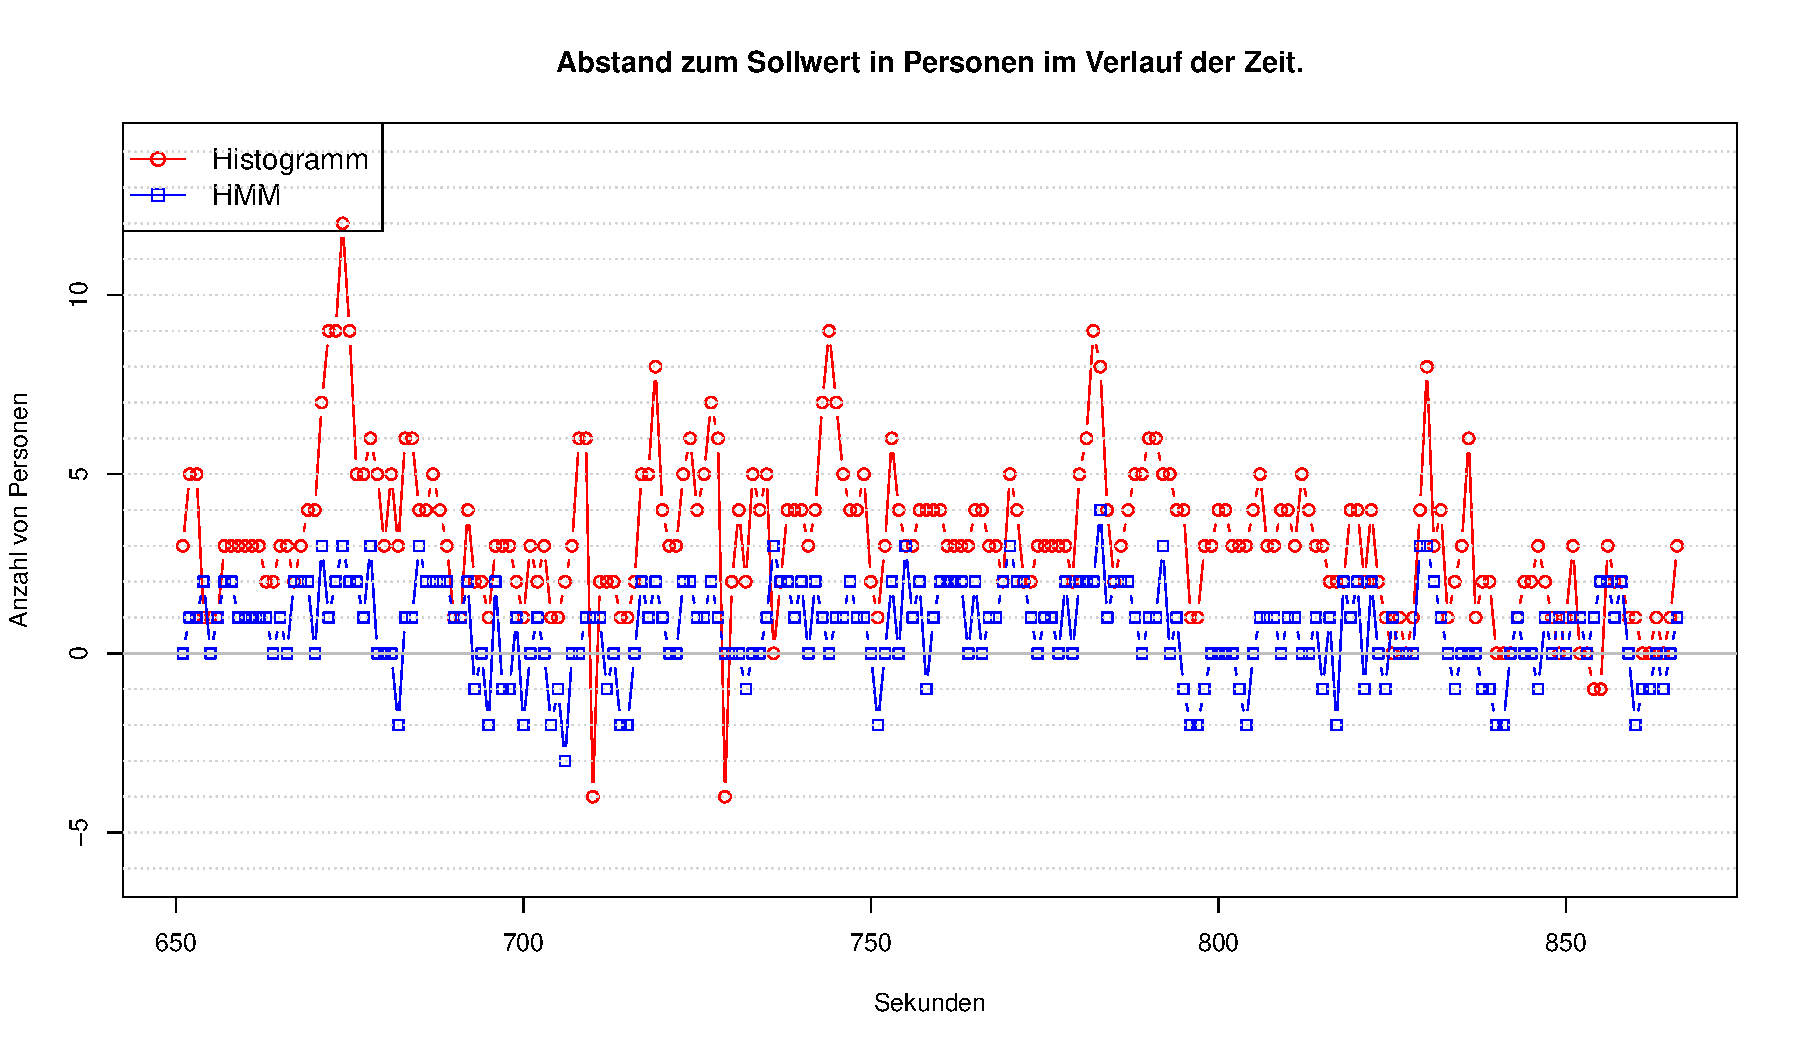
\includegraphics[width=1\textwidth]{bilder/safest_plot_histo_vs_prelearned_652-end.pdf}
	\caption{Eingang: Histogramm vs. trainiertes HMM, Ausschnitt Sekunde 651-Ende}
	\label{fig:Eingang-teil}
\end{figure}

In der Abbildung \ref{fig:Eingang-gesamt} erkennt man anhand der deutlich stärkeren Abweichung, dass beide Algorithmen Probleme mit der zuverlässigen Vordergrundextraktion haben.\\
Während in der ersten Hälfte des Videos der Histogramm-basierte Algorithmus noch Vorteile hat (relativ viele korrekte Anzeigen, der HMM-basierte Algorithmus erkennt meist eine Person zu viel), ist der HMM-basierte Algorithmus in der zweiten Hälfte des Videos (ab etwa Sekunde 450) deutlich besser. Wie der Grafik \ref{fig:Eingang-teil} zu entnehmen ist, existieren wesentlich weniger Ausreißer und das Ergebnis ist insgesamt auch viel dichter am korrekten Wert.\\

\subsection{Diskussion}
\label{sec:diskuss}
Aus den vorangehenden Grafiken kann man ablesen, dass beide Algorithmen grundsätzlich dazu geeignet sind, Vorder- von Hintergrund zu trennen. Sie besitzen jedoch Vor- und Nachteile in bestimmen Szenerien. Genau jene Unterschiede und Details müssen näher beschrieben und erklärt werden.

Wie aus Grafik \ref{fig:Eingang-gesamt} und \ref{fig:Eingang-teil} (Eingang) hervorgeht, besitzt der von uns entwickelte HMM-basierte Algorithmus besonders bei schwierigen, das heißt heterogenen, Hintergründen Vorteile bei der Erkennung. Trotz des hellen Hintergrunds, der viele Kanten und der häufigen Neukalibrierung der Kamera ist eine Erkennung mit kaum Ausreißern möglich. Dies liegt darin begründet, dass sich die Dynamik und die Veränderungen des Videobildes durch einen langen Lernprozess mitteln und des Weiteren Vordergrund nicht anhand von einfachen Grauwerten sondern anhand der komplexen (von uns eingeführten) Emissionen und den Übergängen zwischen ihnen erkannt wird.

Liegt jedoch ein homogener Hintergrund vor, so kann gesagt werden, dass beide Algorithmen gut funktionieren, jedoch ist in dieser Situation der Histogramm-basierte Algorithmus besser. Das liegt daran, dass der Hintergrund einen bestimmten Grauwert besitzt und auch Personen in ein ganz spezielles Intervall der Grauwerte fallen. Demnach arbeitet hier der Histogramm-basierte Algorithmus sehr effizient, unser Algorithmus unterliegt in dieser Domäne.

Den größten Vorteil hat der Histogramm-basierte Algorithmus bei der Performance: während dieser mit 22-25 fps eine flüssige Videodarstellung ermöglicht, lief der HMM-basierte Algorithmus nur mit ca. 10-12 fps. Hier wäre also noch Potential zur Verbesserung bei unserem Algorithmus.\\
Leider hat sich im Laufe des Projekts gezeigt, dass CvHMM sehr ineffizient auf einzelne Daten zugreift und die Ursache hierfür ist. Dies konnten wir mit Hilfe von Callgrind (Teil von Valgrind) nachweisen. Ein weiterer großer Nachteil von CvHMM ist, dass nur eine begrenzte Anzahl von Algorithmen Angeboten wird. Es fehlt der Forward-Algorithmus, den wir mit Hinblick auf die Performance dem ineffizienteren Viterbi-Algorithmus vorziehen würden. Auch haben die Veränderungen an der Netzwerktopologie keine Veränderungen am Resultat ergeben, was wir auf die Implementierung des Baum-Welch-Algorithmus in CvHMM zurückführen. Somit konnte nicht überprüft werden, ob die von uns verwendeten zwei Zustände optimal waren.

Zusätzlich sei angemerkt, dass außer im Falle der Grafik \ref{fig:Innenhof} (Innenhof) die Verläufe beider Graphen sehr ähnlich sind. Dies legt nahe, dass die vorliegenden Fehler eine gemeinsame Ursache besitzen. Diese Ursache konnte von uns teilweise lokalisiert werden: das Clustering, welches markierten Vordergrund in die Anzahl von Personen übersetzt, ist oft zu großzügig. Wir konnten beobachten, dass bei den Tegel- und Eingang-Videos einzelne Personen in zwei oder mehr Cluster (Personen) geteilt werden.

Unseren Ergebnissen nach bewerten wir unser Algorithmus als einen allgemein einsatzfähigen Algorithmus, der in allen Szenerien gut genug ist (ein \glqq allrounder\grqq{}) der gegenüber dem spezialisierten Histogramm-basierten Ansatz in manchen Szenerien besser, in manchen schlechter abschneidet, aber stets gut genug ist.
